\subsection{Protótipo de Baixa Fidelidade}

\begin{figure}[h]
   \centering
   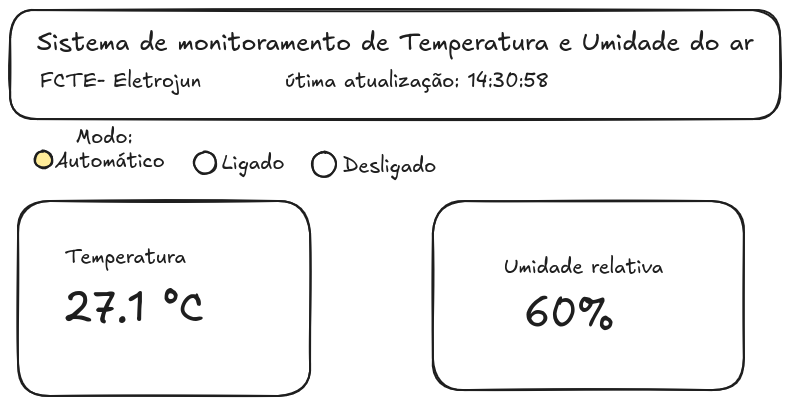
\includegraphics[width=0.8\textwidth]{imagens/Interface_baixa_fidelidade.png} 
    \caption{Protótipo de baixa fidelidade da interface do usuário}
\end{figure}

O protótipo de baixa fidelidade da interface foi desenvolvido com o objetivo de representar a estrutura inicial do sistema de monitoramento de temperatura e umidade do ar. A interface apresenta, de forma simplificada, a organização dos principais elementos necessários para a interação do usuário com o sistema.

Na parte superior, são exibidas informações gerais, como o título do sistema e o horário da última atualização dos dados, permitindo ao usuário identificar rapidamente o estado atual do monitoramento. Logo abaixo, encontra-se a seção de controle de modos de operação, composta pelas opções \textit{Automático}, \textit{Ligado} e \textit{Desligado}, possibilitando a interação direta com o sistema.

A interface também apresenta dois blocos principais de visualização de dados: um destinado à temperatura, exibida em graus Celsius, e outro à umidade relativa do ar, exibida em porcentagem. Esses elementos foram organizados de forma a facilitar a leitura rápida e intuitiva das informações.

O protótipo não contempla aspectos visuais detalhados, como cores definitivas ou estilização avançada, focando apenas na disposição dos componentes e na usabilidade. Dessa forma, ele permite validar a coerência entre a interface proposta e os requisitos funcionais definidos, especialmente aqueles relacionados ao monitoramento em tempo real e ao controle dos modos de operação via interface web.

\subsection{Protótipo de Alta Fidelidade}

\begin{figure}[H]
   \centering
   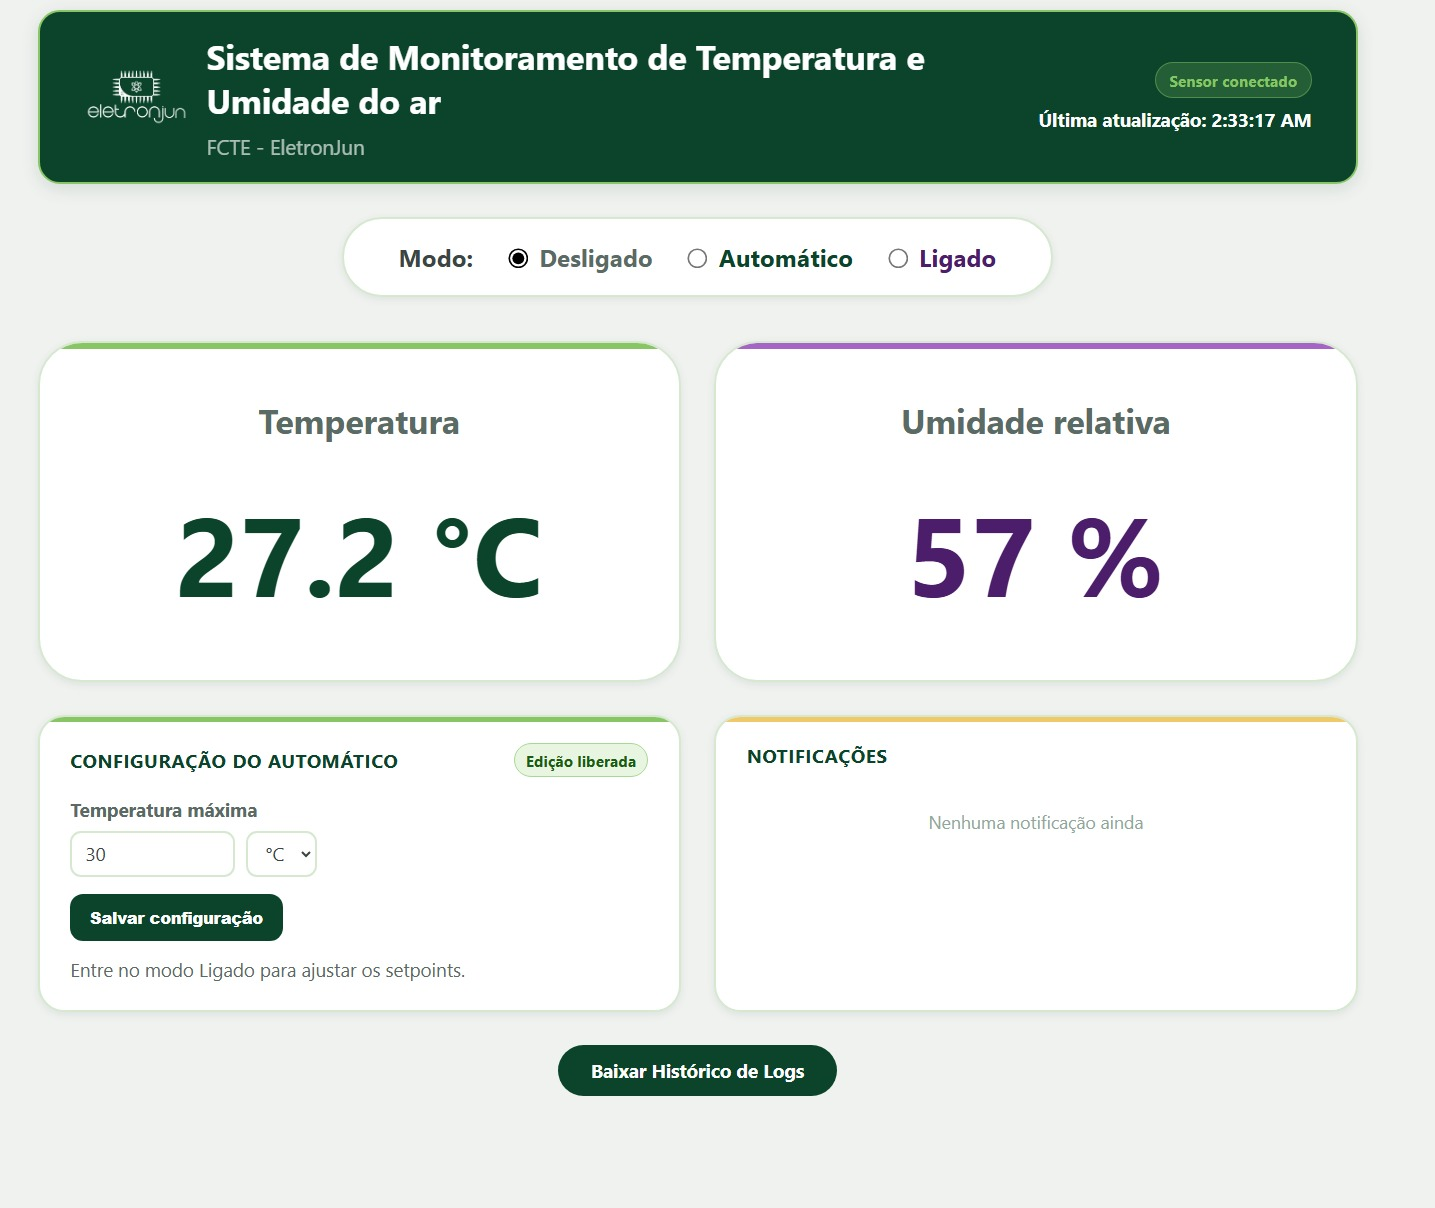
\includegraphics[width=0.5\textwidth]{imagens/sistema_celsius.jpeg} 
    \caption{Protótipo de alta fidelidade da interface do usuário (versão Celsius)}
\end{figure}

\begin{figure}[H]
   \centering
   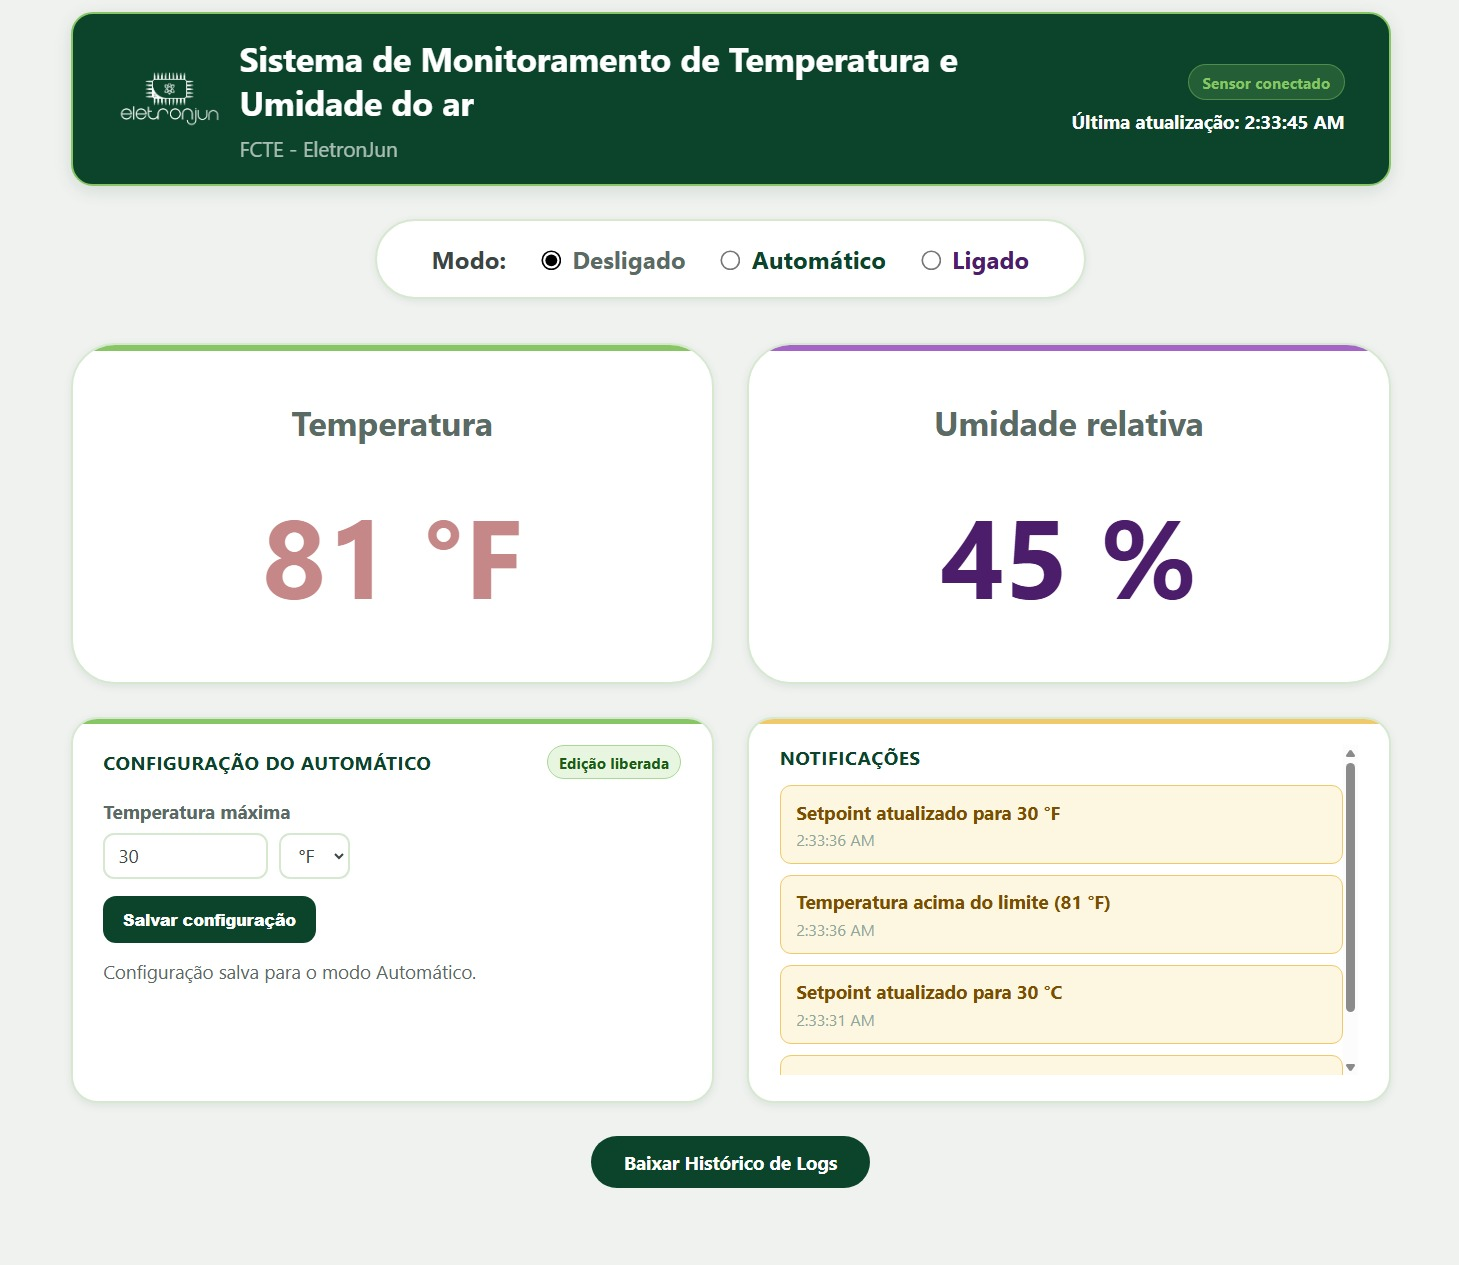
\includegraphics[width=0.5\textwidth]{imagens/sistema_f.jpeg} 
    \caption{Protótipo de alta fidelidade da interface do usuário (versão Fahrenheit)}
\end{figure}

O protótipo de alta fidelidade da interface foi desenvolvido com o objetivo de melhoria e implementação do requisito de hitórico de temperaturas. A interface apresenta, de forma sofisticada, a organização de todos os elementos necessários para a utilização do sistema pelo usuário.

Na parte superior, temos o cabeçalho seguido de informações gerais sobre o projeto, como o título do sistema e o horário da última atualização de temperatura, permitindo o usuário ter conhecimento das informações adquiridas. Abaixo, se encontra a seção de automatização de operação, com as opções \textit{Automático}, \textit{Ligado} e \textit{Desligado}, realizando assim as interações com o sistema.

A interface também apresenta quatro blocos: um para registrar as medições de temperatura, exibida em graus Celsius ou graus Fahrenheit, outro para representar a umidade relativa do ar, exibida em porcentagem, outro para descrever o índice de calor, que realiza uma média do registro das temperaturas, e o último que se trata de um gráfico que mostra a variação das temperaturas e ao lado existe uma parte de alertas, onde o sistema alerta quando a temperatura passa de 28°C. 

Na parte inferior, temos um botão que gera o Histórico de Logs, em um arquivo de texto (.txt), para que o usuário tenha registrado todas as mudanças de temperatura que o sensor registrou.

O protótipo de alta fidelidade passou por melhorias, como a implementação de aspectos visuais, como as cores, a temperatura que quando passa de 28°C o texto pisca, indicando que passou do limite estabelecido, também se tornou funcional os botões de operação, que antes eram apenas esboço do protótipo, e foi realizada a conexão hardware-software, permitindo medições reais de temperatura.
